\subsection*{Ejercicio 5. Denoising mediante Análisis Multirresolución (DWT)} %

Aqui le puse ruido gaussiano al electrocardiograma para simular como si la medición estuviera contaminada por algún equipo electrónico y con este me dediqué a limpiarla usando \textit{Wavelet Shrinkage}

Aproveché la Transformada Ondicular Discreta (DWT) con la familia ortogonal \textbf{Daubechies 4 (db4)}, llevándola hasta un nivel de descomposición $L=4$.

\begin{figure}[H]
    \centering
    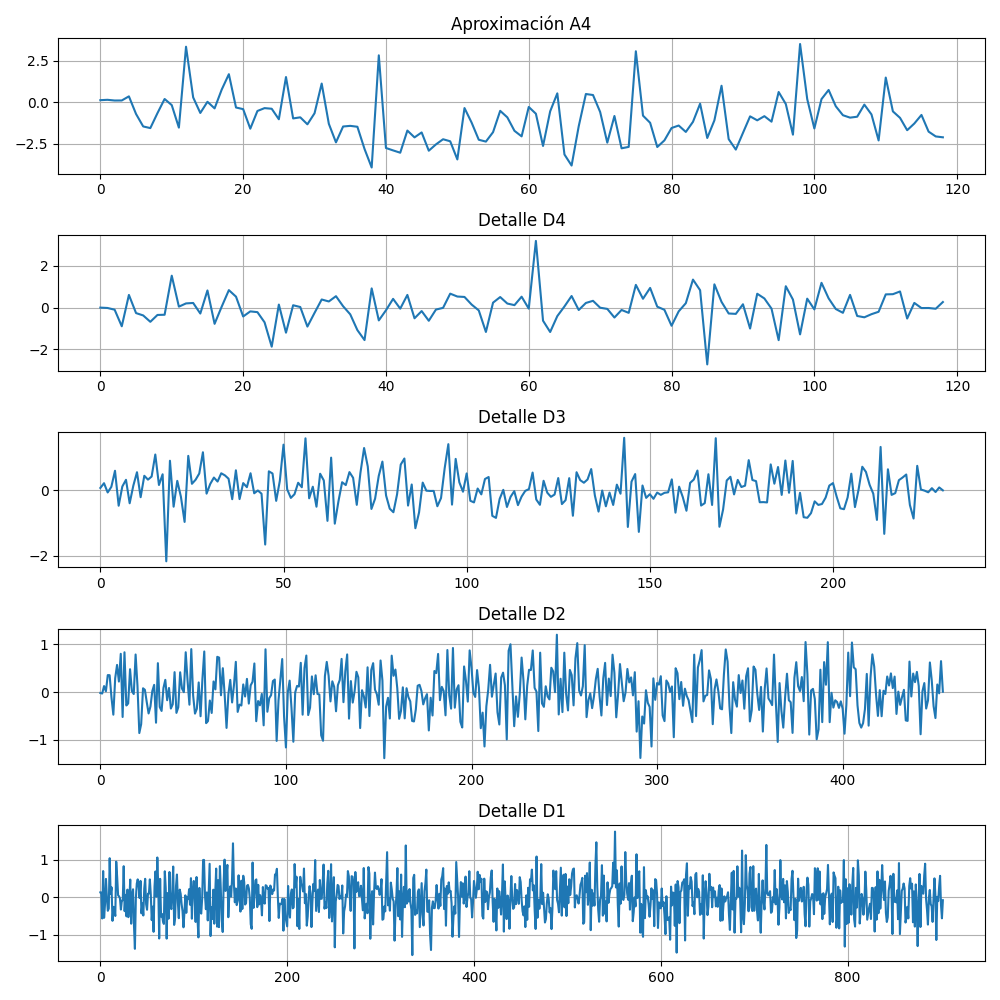
\includegraphics[width=0.8\textwidth]{figuras/ej5_coeficientes.png} 
    \caption{Cascada de coeficientes tras DWT (db4, Nivel 4): Aproximación $A_4$ y Detalles $D_4, D_3, D_2, D_1$.}
\end{figure}

Para quitar el ruido pasé todos los coeficientes desde $D_1$ hasta $D_4$ por una Soft Thresholding porque reduce un poco los coeficientes hacia cero
\begin{equation}
    D_{n}^{(soft)} = \text{sign}(D_n) \cdot \max(|D_n| - \lambda, 0)
\end{equation}

Y para el valor del umbral $\lambda$, decidí ocupar el VisuShrink
\begin{equation}
    \lambda = \sigma \sqrt{2 \ln N}
\end{equation}
Donde $N$ es la cantidad de muestras que tiene nuestra señal y $\sigma$ es lo que estimamos de desviación estándar para el ruido. 

Como en un caso real no sabria como es el ruido calculé la desviación estandar ocupando el Estimador Robusto de la Desviación Absoluta Mediana usando $D_1$
\begin{equation}
    \sigma = \frac{\text{mediana}(|D_1|)}{0.6745}
\end{equation}
El nivel $D_1$ casi toda la información que atrapamos es ruido gaussiano de alta frecuencia que inyectamos al principio, por lo que la constante solo sirve para calibrar el MAD y que funcione como un estimador para la distribución gaussiana

\vspace{0.5cm}
\noindent \textbf{4. Reconstrucción de la Señal (IDWT)} %

Como paso final, regresé al dominio del tiempo con la DWT inversa (IDWT). Para reconstruirla, junté los coeficientes de aproximación que dejamos intactos ($A_4$) con los de detalle que acababa de umbralizar.

\begin{figure}[H]
    \centering
    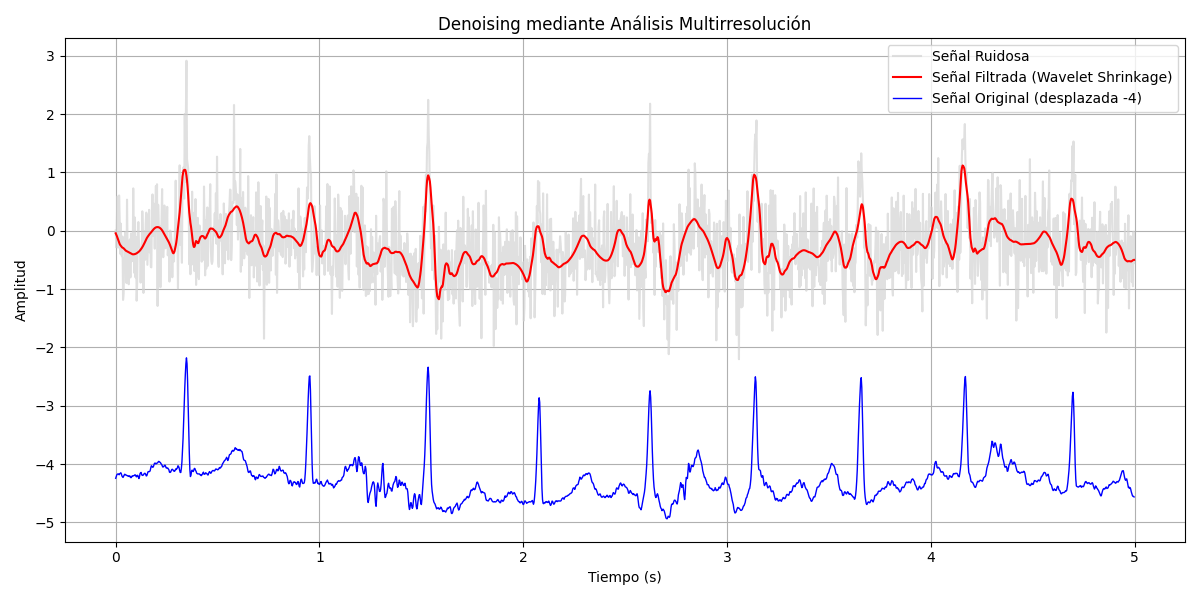
\includegraphics[width=1\textwidth]{figuras/ej5_denoising.png} 
    \caption{Superposición comparativa: Señal ruidosa, señal filtrada mediante Wavelet Shrinkage y la señal original (desplazada en el eje Y para mejor apreciación).}
\end{figure}

Notesé que es un filttrado bastante eficiente ya que si por otro lado se hubiera ocupado un filtro pasa-bajas de Fourier la señal se hubiera dejado irreconocible los picos de los latidos ya que se llevaría componentes de alta frecuencia que sí pertenecen al corazón y con Wavelet Shrinkage se conservan los bordes y transitorios tan marcados del electrocardiograma eliminando la estática
